\documentclass[12pt, a4paper, oneside]{ctexart}
\usepackage{amsmath, amsthm, amssymb, bm, xcolor, tikz, framed, graphicx, hyperref, mathrsfs}

\title{Soild State Physics Homework (Week 3-4)}
\author{Tang Yi \\ [学号已脱敏]}
\usepackage[a4paper, left=2cm, right=2cm, top=2cm, bottom=2cm]{geometry}
\linespread{1.3} % 行距更紧凑
\definecolor{shadecolor}{RGB}{241, 241, 255}

\newcounter{problemname}
\newenvironment{problem}
  {\begin{shaded}\stepcounter{problemname}\par\noindent\textbf{题目 \theproblemname. }}
  {\end{shaded}\par}
\newenvironment{solution}
  {\par\noindent\textbf{题目 \theproblemname 的解答. }}
  {\par}
\newenvironment{note}
  {\par\noindent\textbf{题目 \theproblemname 的注记. }}
  {\par}

\begin{document}
\maketitle
\begin{problem}
    对于简单立方晶格，证明密勒指数为 $(h,k,l)$ 的晶面系，面间距 $d$ 满足：

    \[ d^2 = \frac{a^2}{h^2 + k^2 + l^2} \]

    其中 $a$ 为立方边长。
\end{problem}
\begin{solution}
对于简单立方晶格，晶格常数为 $a$。考虑密勒指数为 $(h,k,l)$ 的晶面。根据密勒指数的定义，该晶面在三个坐标轴上的截距分别为
\[
\frac{a}{h},\quad \frac{a}{k},\quad \frac{a}{l}.
\]
因此，该晶面可以写成截距式方程：
\[
\frac{x}{a/h} + \frac{y}{a/k} + \frac{z}{a/l} = 1,
\]
即
\[
hx + ky + lz = a.
\]

更一般地，与其平行的一族晶面可表示为
\[
hx + ky + lz = n a,\quad n \in \mathbb{Z}.
\]

相邻两晶面分别对应 $n$ 和 $n+1$，即
\[
hx + ky + lz = n a, \quad hx + ky + lz = (n+1)a.
\]

两平行平面 $Ax + By + Cz = D_1$ 与 $Ax + By + Cz = D_2$ 之间的距离为
\[
d = \frac{|D_2 - D_1|}{\sqrt{A^2 + B^2 + C^2}}.
\]

因此，相邻两晶面之间的距离为
\[
d = \frac{|(n+1)a - na|}{\sqrt{h^2 + k^2 + l^2}} 
= \frac{a}{\sqrt{h^2 + k^2 + l^2}}.
\]

从而得到
\[
d^2 = \frac{a^2}{h^2 + k^2 + l^2}.
\]

证毕。
\end{solution}
\begin{problem}
    写出体心立方和面心立方晶格结构的金属中，最近邻和次近邻的原子数。若立方边长为 $a$，写出最近邻和次近邻的原子间距。
\end{problem}
\begin{solution}

\textbf{(1) 体心立方晶格（BCC）}

在体心立方结构中，每个原子位于立方体的顶点或体心。

\begin{itemize}
    \item 最近邻原子数：8 \\
    体心原子与8个顶点原子互为最近邻。
    
    最近邻距离为体对角线的一半：
    \[
    d_1 = \frac{\sqrt{3}}{2}a
    \]
    
    \item 次近邻原子数：6 \\
    次近邻为沿立方体棱方向的原子。
    
    次近邻距离为：
    \[
    d_2 = a
    \]
\end{itemize}

\vspace{0.5em}

\textbf{(2) 面心立方晶格（FCC）}

在面心立方结构中，每个原子位于顶点和各个面的中心。

\begin{itemize}
    \item 最近邻原子数：12 \\
    每个原子与同一面及相邻面的原子构成最近邻关系。
    
    最近邻距离为面对角线的一半：
    \[
    d_1 = \frac{\sqrt{2}}{2}a
    \]
    
    \item 次近邻原子数：6 \\
    次近邻为沿立方体棱方向的原子。
    
    次近邻距离为：
    \[
    d_2 = a
    \]
\end{itemize}

\end{solution}


\newpage
\begin{problem}
    画出体心立方和面心立方晶格结构的金属在 $(100)$，$(110)$，$(111)$ 面上的原子排列。
\end{problem}

\begin{solution}

    如上
    \begin{figure}
    \centering
    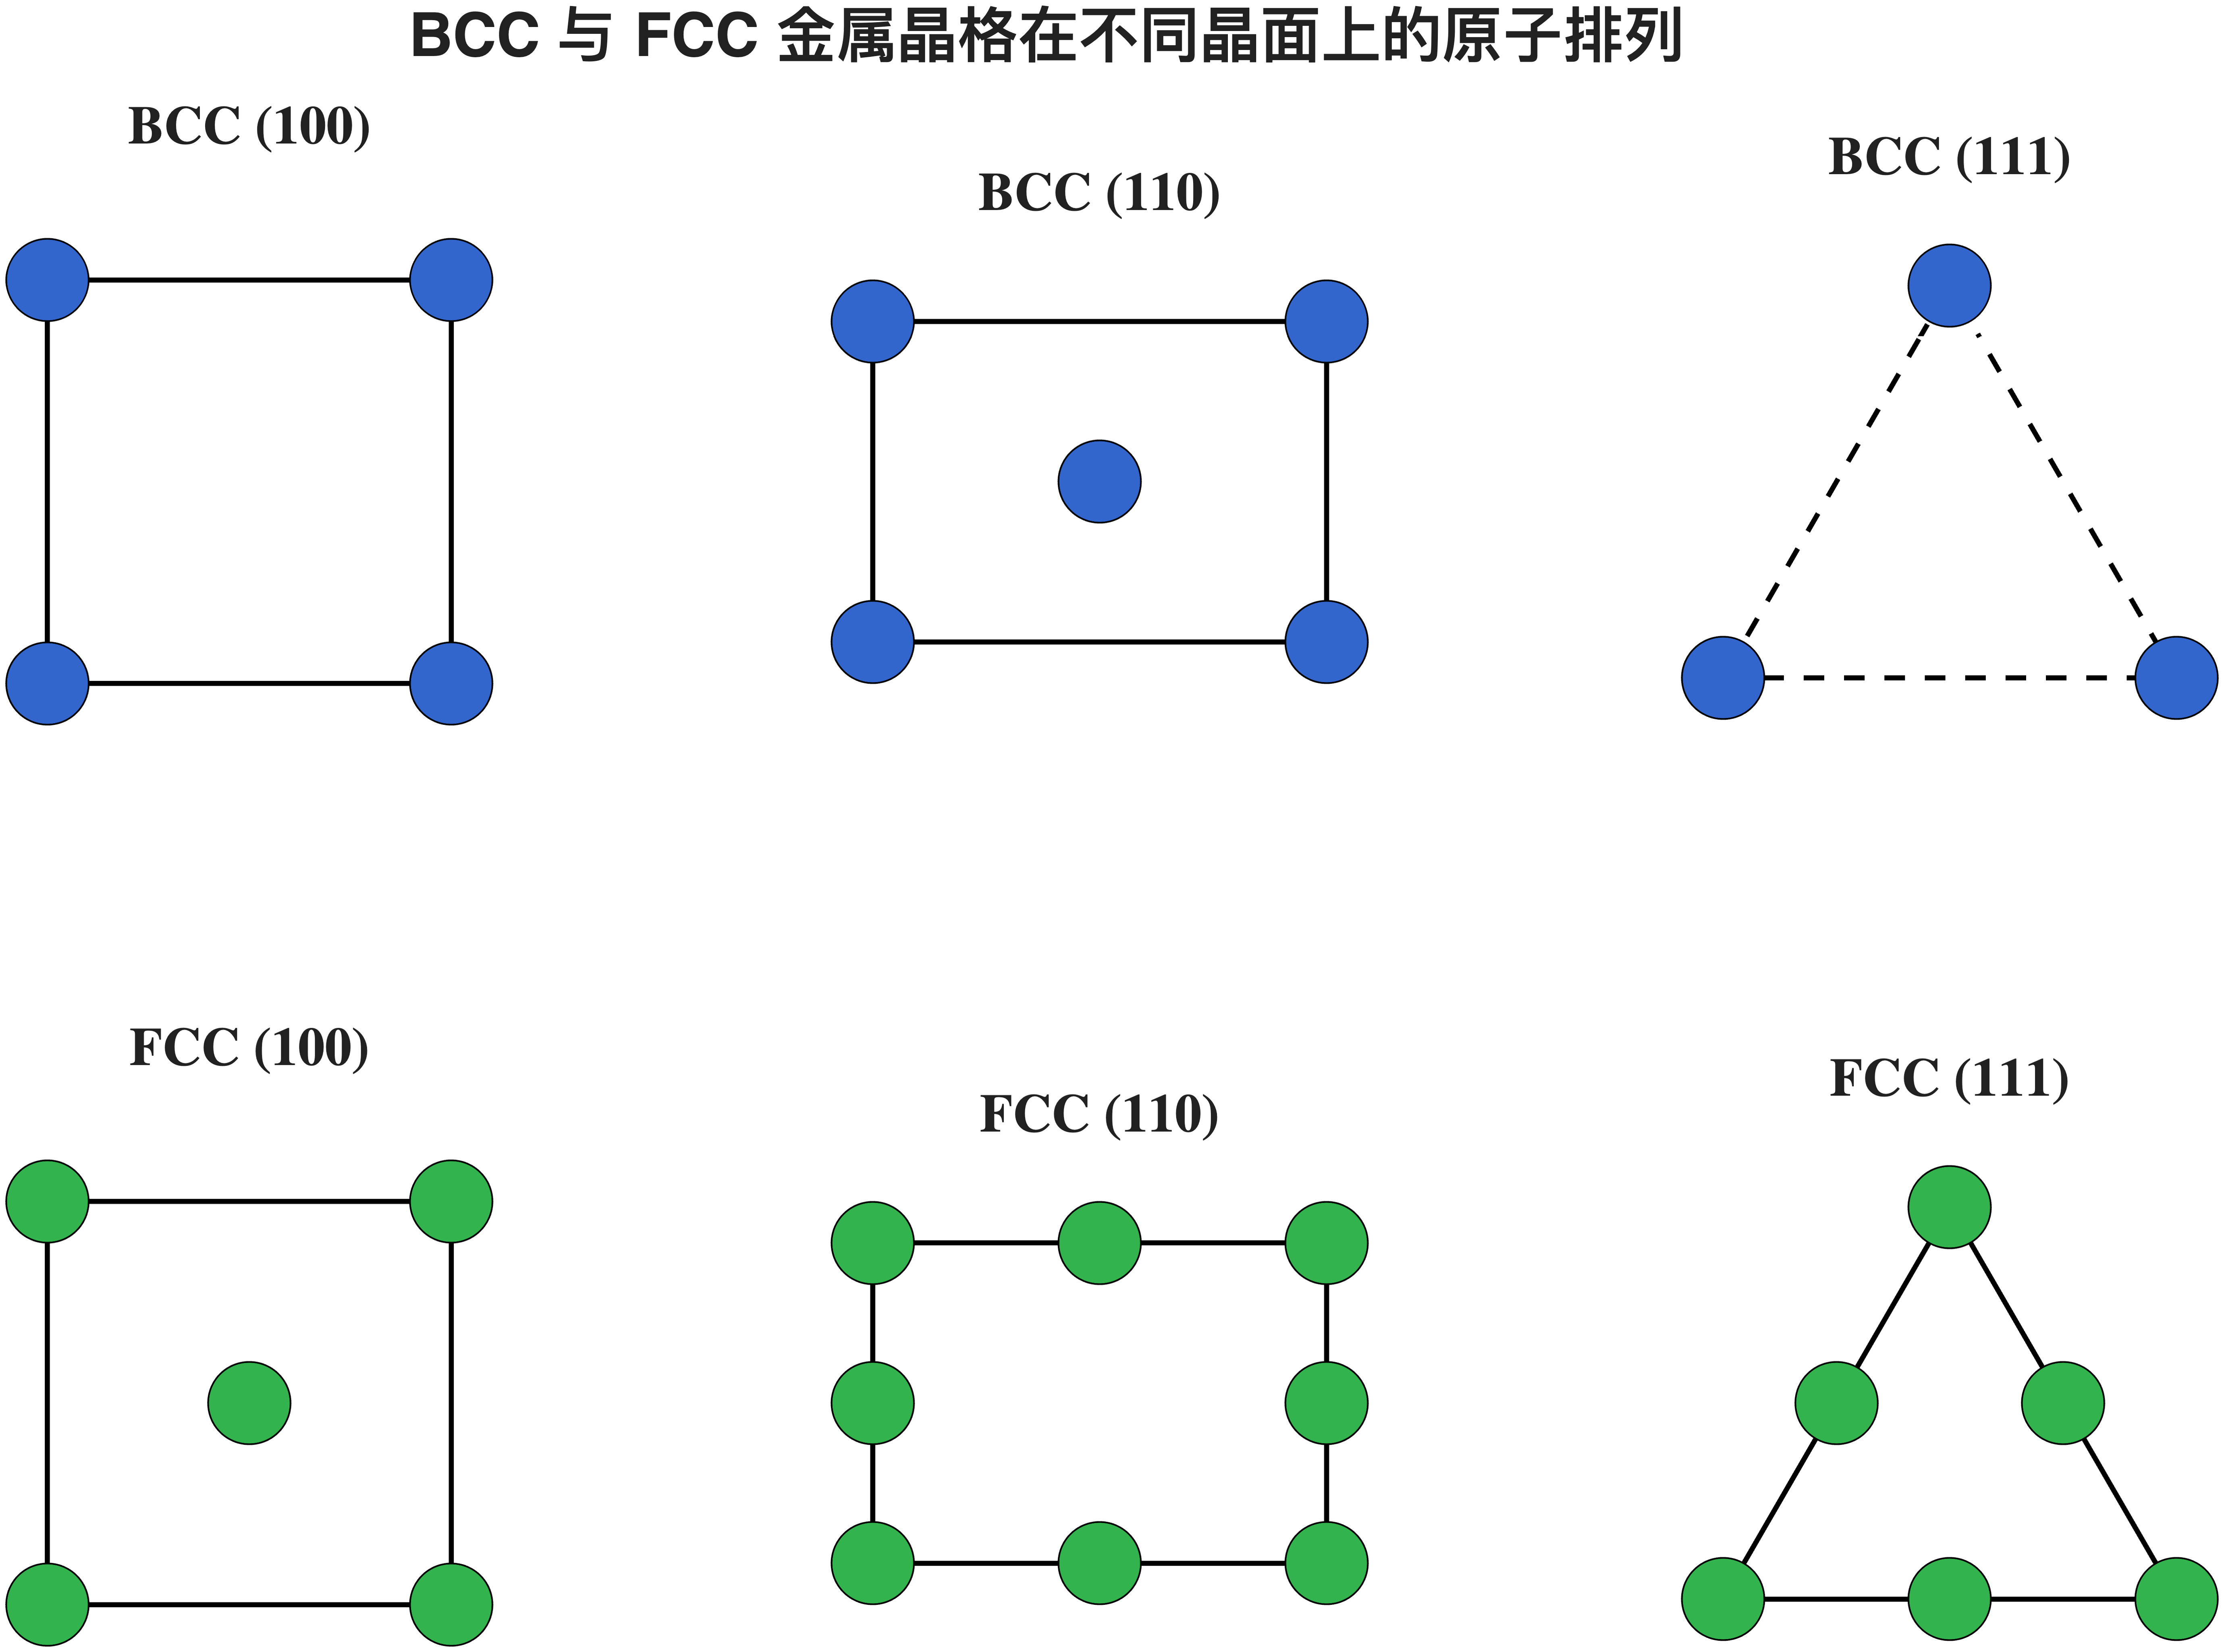
\includegraphics[width=0.8\textwidth]{111.png}
    \end{figure}
\end{solution}



\begin{problem}
    指出立方晶格 $(111)$ 面与 $(100)$ 面，$(111)$ 面与 $(110)$ 面的交线的晶向。
\end{problem}

\begin{solution}
立方晶格中，晶面 $(hkl)$ 的法向量为 $(h, k, l)$。因此：
对于立方晶格，晶面 $(hkl)$ 的法向量可以用 $[hkl]$ 表示。  
两平面交线的方向 $\mathbf{d}$ 垂直于两平面的法向量，即
\[
\mathbf{d} = \mathbf{n}_1 \times \mathbf{n}_2,
\]
其中 $\mathbf{n}_1$ 和 $\mathbf{n}_2$ 分别是两平面的法向量。

\subsubsection*{$(111)$ 面与 $(100)$ 面的交线}

\[
\mathbf{n}_1 = [1,1,1], \quad \mathbf{n}_2 = [1,0,0]
\]

交线方向为：
\[
\mathbf{d} = \mathbf{n}_1 \times \mathbf{n}_2
= 
\begin{vmatrix}
\mathbf{i} & \mathbf{j} & \mathbf{k} \\
1 & 1 & 1 \\
1 & 0 & 0
\end{vmatrix}
= [0,1,-1]
\]

因此晶向为：
\[
[0,1,\overline{1}]
\]

\subsubsection*{$(111)$ 面与 $(110)$ 面的交线}

\[
\mathbf{n}_1 = [1,1,1], \quad \mathbf{n}_2 = [1,1,0]
\]

交线方向为：
\[
\mathbf{d} = \mathbf{n}_1 \times \mathbf{n}_2
=
\begin{vmatrix}
\mathbf{i} & \mathbf{j} & \mathbf{k} \\
1 & 1 & 1 \\
1 & 1 & 0
\end{vmatrix}
= [-1,1,0]
\]

因此晶向为：
\[
[\overline{1},1,0]
\]
\end{solution}

\begin{problem}
    证明两种一价离子组成的一维晶格的马德隆常数为
    \[ \alpha = 2 \ln 2 \]
\end{problem}

\begin{solution}
    考虑一维交替排列的两种一价离子晶格，离子间距为 $a$，离子序列为：
\[
\cdots - + - + - + - \cdots
\]

对任意一个正离子，其与其他所有离子的相互作用能（忽略 $1/(4\pi\varepsilon_0)$ 因子）为：
\[
U = - \frac{q^2}{a} \sum_{n=1}^{\infty} \frac{(-1)^n}{n} = - \frac{q^2}{a} \alpha
\]

因此马德隆常数为：
\[
\alpha = \sum_{n=1}^{\infty} \frac{(-1)^n}{n} = 1 - \frac{1}{2} + \frac{1}{3} - \frac{1}{4} + \cdots
\]

这是一个已知的交错调和级数，其和为：
\[
\sum_{n=1}^{\infty} \frac{(-1)^{n+1}}{n} = \ln 2
\]

考虑到每个离子左右两侧都有相同贡献，因此总马德隆常数为：
\[
\alpha = 2 \ln 2
\]
\end{solution}

\begin{problem}
    讨论使离子电荷加倍所引起的对 $\text{NaCl}$ 晶格常数及结合能的影响。（排斥势看作不变）
\end{problem}

\begin{solution}
    NaCl 晶格结合能公式为：
\[
U = - \frac{\alpha q^2}{4 \pi \varepsilon_0 a} + \frac{B}{a^n},
\]
其中 $\alpha$ 为马德隆常数，$a$ 为晶格常数，$B,n$ 为排斥势参数。

晶格平衡条件：
\[
\frac{dU}{da} = 0 \quad \Rightarrow \quad \frac{\alpha q^2}{4 \pi \varepsilon_0 a_0^2} - n \frac{B}{a_0^{n+1}} = 0 \quad \Rightarrow \quad B = \frac{\alpha q^2}{4 \pi \varepsilon_0 n} a_0^{n-1}.
\]

若离子电荷加倍 $q' = 2q$，排斥势不变，则新的平衡晶格常数 $a'$ 满足：
\[
\frac{\alpha (2q)^2}{4 \pi \varepsilon_0 a'^2} - n \frac{B}{a'^{\,n+1}} = 0.
\]

代入 $B$：
\[
\frac{4 \alpha q^2}{4 \pi \varepsilon_0 a'^2} - n \frac{\alpha q^2}{4 \pi \varepsilon_0 n} \frac{a_0^{\,n-1}}{a'^{\,n+1}} = 0
\quad \Rightarrow \quad a'^{\,n-1} = \frac{1}{4} a_0^{\,n-1} 
\quad \Rightarrow \quad a' = a_0 \, 4^{-1/(n-1)}.
\]

结合能为：
\[
U' = - \frac{\alpha (2q)^2}{4 \pi \varepsilon_0 a'} \left(1 - \frac{1}{n}\right) 
= - \frac{4 \alpha q^2}{4 \pi \varepsilon_0 a'} \left(1 - \frac{1}{n}\right),
\]
比原来绝对值更大。
\end{solution}
\end{document}